\documentclass[12pt,a4paper]{article}

\usepackage[a4paper,left=3.0cm,right=2.5cm,top=2.5cm,bottom=2.5cm]{geometry}
\usepackage{newtxtext,newtxmath}
\usepackage{setspace}
\usepackage{graphicx}
\usepackage{array}
\usepackage{booktabs}
\usepackage{tabularx}
\usepackage{caption}
\usepackage{titlesec}
\usepackage{amsmath}
\usepackage{eso-pic}
\usepackage{tikz}
\usepackage{algorithm}
\usepackage{algpseudocode}
\usepackage{enumitem}
\usepackage[hidelinks]{hyperref}
\usetikzlibrary{shapes.geometric,arrows.meta,positioning,calc}

\onehalfspacing
\setlength{\parskip}{4pt}
\setlength{\parindent}{0pt}
\graphicspath{{figures/}}

\titleformat{\section}{\fontsize{14}{17}\selectfont\bfseries}{\thesection.}{0.6em}{}
\titleformat{\subsection}{\fontsize{12}{15}\selectfont\bfseries}{\thesubsection}{0.6em}{}
\titlespacing*{\section}{0pt}{14pt}{6pt}
\titlespacing*{\subsection}{0pt}{10pt}{4pt}

\captionsetup{font=small,labelfont=bf,justification=centering}
\renewcommand{\contentsname}{Index}
\setcounter{tocdepth}{1}
\renewcommand{\refname}{References}

\AddToShipoutPictureBG{%
  \begin{tikzpicture}[remember picture,overlay]
    \draw[line width=0.6pt] ([shift={(1.5cm,1.5cm)}]current page.south west) rectangle ([shift={(-1.5cm,-1.5cm)}]current page.north east);
  \end{tikzpicture}}

\tikzset{
  block/.style={rectangle,draw,minimum height=1.0cm,minimum width=2.2cm,align=center,font=\small},
  sum/.style={circle,draw,minimum size=0.7cm,inner sep=0pt,font=\small},
  proc/.style={rectangle,draw,rounded corners=2pt,minimum height=0.8cm,text width=4.2cm,align=center,font=\small},
  dec/.style={diamond,draw,aspect=2.2,text width=3.0cm,align=center,inner sep=1pt,font=\small},
  term/.style={rectangle,draw,rounded corners=8pt,minimum height=0.8cm,text width=3cm,align=center,font=\small},
  arr/.style={-{Latex[length=2mm]}}
}

\newcommand{\projtitle}{Conveyor Motor Speed Control: Bang-Bang, PWM and PID}

\begin{document}

% ---------------- Title page ----------------
\thispagestyle{empty}
\begin{center}
\IfFileExists{figures/upes_logo.png}{\includegraphics[width=5.5cm]{upes_logo.png}\\[0.3cm]}{\vspace{2.6cm}}
{\bfseries School of Computer Science, UPES, Dehradun}\\[1.2cm]
A Project Report on\\[0.5cm]
{\fontsize{19}{23}\selectfont\bfseries Conveyor Motor Speed Control:\\[0.15cm] Bang-Bang, PWM and PID}\\[1.2cm]
{\small Submitted for the course}\\[0.2cm]
{\bfseries CSAI4014 Algorithms for Intelligent Systems and Robotics}\\[0.2cm]
B.Tech CSE (AI \& ML), Semester VII\\[1.0cm]
\begin{tabular}{@{}ll@{}}
\textbf{Project No.:} & P15 \\
\textbf{Group No.:}   & G07 \\
\textbf{Batch:}       & B1 \\
\end{tabular}\\[1.0cm]
{\bfseries Submitted by}\\[0.3cm]
\begin{tabular}{|c|l|c|}
\hline
\textbf{S. No.} & \textbf{Name} & \textbf{SAP ID} \\ \hline
1 & Amulya Jain & 500122439 \\ \hline
2 & Aasthik Upadhyay & 500123174 \\ \hline
3 & Krish Manwani & 500123449 \\ \hline
4 & Vanshaj Tiwari & 500123258 \\ \hline
5 & Yash Dagar & 500125147 \\ \hline
\end{tabular}\\[1.0cm]
{\bfseries Submitted to}\\[0.2cm]
Course Faculty, CSAI4014\\
School of Computer Science, UPES, Dehradun\\[0.6cm]
Academic Year 2026-2027 \textbar\ October 2026
\end{center}
\clearpage

% ---------------- Front matter ----------------
\pagenumbering{roman}
\setcounter{page}{1}

\section*{Declaration}
\addcontentsline{toc}{section}{Declaration}
We declare that this project report titled ``\projtitle'' is our own work, carried out for the course CSAI4014 Algorithms for Intelligent Systems and Robotics. The code, results and text are original, and all sources used are cited in the References.

\vspace{0.8cm}
\begin{center}
\begin{tabular}{|l|c|p{4cm}|}
\hline
\textbf{Name} & \textbf{SAP ID} & \textbf{Signature} \\ \hline
Amulya Jain & 500122439 & \\[0.5cm] \hline
Aasthik Upadhyay & 500123174 & \\[0.5cm] \hline
Krish Manwani & 500123449 & \\[0.5cm] \hline
Vanshaj Tiwari & 500123258 & \\[0.5cm] \hline
Yash Dagar & 500125147 & \\[0.5cm] \hline
\end{tabular}
\end{center}

\vspace{0.8cm}
Date: \underline{\hspace{4cm}} \hfill Place: Dehradun
\clearpage

\section*{Abstract}
\addcontentsline{toc}{section}{Abstract}
Roller and belt conveyors are everywhere in warehouses, airports and factories, and almost all of them are driven by an electric motor whose speed must be held constant while the load on the belt changes. This project models a brushed DC motor driving a ten-roller conveyor in the PyBullet physics engine, with rigid load boxes that are transported by roller friction and are dropped onto the belt at chosen moments. Three speed controllers are implemented on exactly the same plant: a hysteresis bang-bang controller, a proportional-duty PWM controller with a 50 Hz carrier, and a PID controller with integrator anti-windup. The motor supply is limited to 24 V, so actuator saturation is part of every experiment. A Python command-line dashboard shows speed, voltage, current and duty cycle live, and a compare mode prints rise time, overshoot, steady-state error, ripple, load dip, recovery time and switching count for the three controllers side by side. The PyBullet plant was validated against the analytical second-order transfer function of the motor-roller system: final speed matched to four digits and the time constant to within 3 percent. Under a three-box load change the PID controller dipped by 0.064 m/s and recovered in 0.12 s, against 0.088 m/s with no settling for bang-bang and 0.158 m/s with a 0.10 m/s permanent offset for PWM. The novelty lies in the contact-based load model, the model-validated plant and the unified metric set used for the comparison.

\textbf{Keywords:} conveyor, DC motor, bang-bang control, PWM, PID, anti-windup, PyBullet.
\clearpage

\tableofcontents
\clearpage

\listoffigures
\addcontentsline{toc}{section}{List of Figures}
\vspace{1cm}
\listoftables
\addcontentsline{toc}{section}{List of Tables}
\clearpage

\section*{Writing Allocation}
\addcontentsline{toc}{section}{Writing Allocation}
\begin{center}
\begin{tabular}{|c|l|p{6.2cm}|c|}
\hline
\textbf{Member} & \textbf{Name and SAP ID} & \textbf{Sections written} & \textbf{Pages} \\ \hline
M1 & Amulya Jain (500122439) & 6, 8 & 5 \\ \hline
M2 & Aasthik Upadhyay (500123174) & 5, 12 & 5 \\ \hline
M3 & Krish Manwani (500123449) & 3, 4 & 5 \\ \hline
M4 & Vanshaj Tiwari (500123258) & 7, 9 & 6 \\ \hline
M5 & Yash Dagar (500125147) & Abstract, 1, 2, References, Appendix & 5 \\ \hline
All & Every member & 10 (own row), 11 (own reflection), Declaration & - \\ \hline
\end{tabular}
\end{center}
\clearpage

% ---------------- Main matter ----------------
\pagenumbering{arabic}
\setcounter{page}{1}

\section{Introduction}

A conveyor is the simplest material-handling machine there is: a moving surface that carries objects from one place to another. Belt conveyors move bulk material in mines and ports, roller conveyors move parcels in sorting hubs and e-commerce warehouses, and short modular conveyors link the stations of almost every assembly line. In all of these the surface speed of the conveyor is a process variable that must be controlled. Downstream machines such as scanners, labellers, pick-and-place robots and sorter diverters are timed on the assumption that the belt moves at a known speed, and a conveyor that slows under load or surges when it is unloaded breaks the spacing between items, causes mis-sorts and, in the worst case, jams \cite{cema}.

The drive of a conveyor is an electric motor, and in small and medium machines it is very often a brushed or brushless DC motor fed from a DC bus through a switching power stage \cite{hughes}. The problem of holding the belt speed constant is therefore a motor speed control problem, and it has the three features that make motor control interesting in practice. First, the load changes: a parcel landing on the belt adds mass that has to be accelerated and adds friction that has to be overcome, while a parcel leaving the belt removes them again. Second, the actuator saturates: the supply voltage, and therefore the torque, is limited, so a controller can ask for more than the drive can give. Third, the actuator is usually switched: power electronics do not deliver a smooth voltage but a train of pulses, and the motor inductance and inertia average those pulses out \cite{mohan}.

The same problem appears far outside conveyors. The traction drive of an electric vehicle, the spindle of a machine tool, the fan of a ventilation system and the wheel motors of a mobile robot are all speed-controlled electric motors facing load changes and saturation \cite{leonhard}. The control strategies used for them form a ladder of increasing sophistication: on-off (bang-bang) control, as in a thermostat or a contactor; pulse-width modulation (PWM) with a duty cycle set by some rule; and closed-loop proportional-integral-derivative (PID) control, which is the workhorse of industrial drives \cite{astrom-hagglund}. Understanding what each strategy gives and what it costs, on one plant and one set of disturbances, is the purpose of this project.

Building and instrumenting a real conveyor drive would take more time and money than a course project allows, so the plant is built in PyBullet \cite{pybullet}, an open-source rigid-body physics engine with a Python interface. PyBullet is attractive here for a reason that is easy to overlook: the load boxes are real rigid bodies that sit on the rollers, are accelerated by Coulomb friction, bounce when they are dropped, and exert reaction torques on the rollers. The load disturbance is therefore not a number injected into an equation but a consequence of contact physics, which is much closer to how a real conveyor is loaded. The motor itself is modelled analytically, because PyBullet has no electrical domain, and the two are coupled every millisecond.

The deliverable is a Python command-line tool. One command starts the simulation with the chosen controller, shows a live text dashboard of speed, voltage, current, torque and duty cycle, and prints a set of response metrics when the run ends. Another command runs the three controllers back to back on an identical scenario and prints the metrics in one table. Every figure in this report was produced by a script in the repository from those same runs, so every number here can be regenerated from the code.

The remainder of the report is organised as the course template requires. Section 2 states the problem and the objectives. Section 3 reviews the literature and what industry does today. Section 4 states the novelty. Section 5 maps the work to the AISR syllabus and derives the theory. Sections 6 to 8 describe the system design, the algorithms and the simulation setup. Section 9 presents and discusses the results. Sections 10 to 12 cover contributions, co-learning and conclusions, followed by the references and the appendix with links and logs.

\section{Problem Statement and Objectives}

\textbf{Problem statement.} Model a DC motor driving a conveyor, compare bang-bang, PWM and PID control of the belt speed under load changes and actuator saturation, and run the whole thing from a Python command-line dashboard.

\textbf{Objectives.} The following objectives were set at the first meeting and each one is measurable in the results of Section 9.
\begin{enumerate}[nosep]
  \item Build a conveyor of ten driven rollers with rigid load boxes in PyBullet, and a brushed DC motor model with armature resistance, inductance, back-EMF and a 24 V supply limit, coupled to the rollers at 1 kHz.
  \item Validate the simulated plant against the analytical transfer function from voltage to belt speed: the open-loop final speed must agree within 1 percent and the time constant within 10 percent.
  \item Implement bang-bang, PWM and PID speed controllers behind one common interface, and hold a 0.5 m/s setpoint with three 1 kg boxes on the belt. The PID controller must show a steady-state error below 0.005 m/s and an overshoot below 5 percent.
  \item Quantify the response to a load change (three boxes dropped at once onto a running belt) and to actuator saturation (setpoints at and beyond the motor's top speed), and show the effect of integrator anti-windup.
  \item Provide a command-line dashboard that refreshes at 10 Hz in simulated time and a compare mode that reports rise time, overshoot, steady-state error, ripple, load dip, recovery time, mean voltage and switching count for all three controllers.
\end{enumerate}

\textbf{Assumptions.} The rollers are rigid and all sit on one shaft, so they share the motor torque equally and turn at the same speed. There is no belt elasticity or slip between rollers and belt because the boxes ride directly on the rollers. The speed sensor is ideal: the belt speed is read from the physics engine without noise or delay. The drive is unidirectional, the voltage command is in $[0, 24]$ V, and a command of 0 V shorts the armature, which is the ``brake'' mode of an H-bridge. Bearing friction is viscous.

\textbf{Limits.} The PWM carrier is 50 Hz, two orders of magnitude lower than real motor drivers, because the physics step is 1 ms; the consequences are discussed in Section 9. Motor rotor inertia and gearbox are neglected. Temperature effects on winding resistance are ignored.

\section{Literature and Industry Review}

\subsection{Motor speed control in textbooks}

The brushed DC motor is the standard first example of an electromechanical system in control textbooks. Ogata \cite{ogata} and Franklin, Powell and Emami-Naeini \cite{franklin} both derive the armature-controlled DC motor as a second-order system whose transfer function from voltage to shaft speed has one electrical and one mechanical pole, and both use it to introduce step response, time constants, root locus and PID design. Åström and Murray \cite{astrom-murray} use the same model to discuss the limits imposed by actuator saturation, and devote a section to integrator wind-up, the phenomenon by which an integral controller keeps accumulating error while the actuator is pinned at its limit and then overshoots badly once the limit is released. Hughes and Drury \cite{hughes} treat the motor from the drive engineer's point of view: torque-speed curves, the role of back-EMF as a natural speed feedback, and the reason that DC drives are fed by chopper circuits rather than by linear amplifiers. Krishnan \cite{krishnan} and Leonhard \cite{leonhard} give the full industrial picture, where a fast inner current loop is wrapped by a slower speed loop, and PWM is simply the way the current loop's voltage demand is realised.

\subsection{Controller families}

\textbf{Bang-bang or on-off control} is the oldest feedback strategy. The actuator has two states and the controller switches between them when the error crosses a threshold. A hysteresis band is added so that the switching frequency stays finite. It is used wherever the actuator can only be switched, for example contactors and relays, and it is also optimal in the time-optimal sense for some problems \cite{astrom-murray}. Its cost is a limit cycle: the controlled variable never rests at the setpoint but oscillates around it at a frequency set by the plant dynamics and the band width, and the actuator switches continuously.

\textbf{Pulse-width modulation} turns a two-state actuator into an effectively continuous one by switching it at a fixed carrier frequency with a variable duty cycle \cite{mohan}. The motor inductance and inertia average the pulses, so the motor sees approximately the mean voltage. In a real drive the carrier is in the range of 2 to 20 kHz. PWM itself is an actuation method, not a control law; the duty cycle still has to come from somewhere. In the simplest arrangement the duty is proportional to the error, which gives a proportional controller with a known steady-state offset.

\textbf{PID control} remains the most used control law in industry; surveys quoted by Åström and Hägglund \cite{astrom-hagglund} put it in more than 90 percent of control loops. The three terms give a direct response to error, elimination of steady-state offset and damping of the transient. The classical tuning rules of Ziegler and Nichols \cite{ziegler} are still the starting point in many plants, although model-based tuning, as used in this project, gives more predictable results when a plant model is available. Practical PID implementations always include some form of anti-windup, and Peng, Vrančić and Hanus \cite{peng} review the main schemes: integrator clamping, back-calculation and conditional integration.

\subsection{What industry does today}

Commercial conveyor drives fall into three groups. Small belt and roller conveyors often use a fixed-speed AC motor and a contactor, which is bang-bang control in all but name: the belt runs or stops. Variable-speed conveyors use a variable frequency drive or a DC chopper drive with a built-in PID speed loop and PWM power stage, which is the PID-over-PWM structure \cite{hughes, leonhard}. Motorised-roller conveyors in modern sorting centres have a brushless DC motor inside each roller with its own driver card and its own speed loop \cite{cema}. In every case the questions are the same as in this project: how fast does the belt recover when a load lands on it, how far does the speed sag, how much does the actuator switch, and what happens when the drive runs out of voltage.

\subsection{Simulation platforms}

PyBullet \cite{pybullet} is a Python binding to the Bullet physics engine. It provides rigid-body dynamics with contact and friction, articulated bodies described in URDF, and joint motor control in position, velocity and torque mode. It is widely used for robot learning research because it is fast enough to run thousands of simulations per hour in headless mode. It has no electrical domain, so motor electrics must be modelled outside it, which is what is done here.

\subsection{The gap}

The textbook treatments compare controllers on a linear plant with the disturbance injected as a torque step. The drive literature assumes a full current loop and a kHz carrier. Neither shows, on one physics-based plant, what happens when each of the three strategies is applied with a slow carrier and a contact-based load, and neither validates the simulated plant against the analytical model before comparing controllers on it. Table \ref{tab:approaches} summarises the approaches and their limitations.

\begin{table}[htbp]
\centering
\caption{Comparison of existing approaches to conveyor and motor speed control}
\label{tab:approaches}
\begin{tabular}{|p{3.6cm}|p{4.4cm}|p{5.0cm}|}
\hline
\textbf{Approach} & \textbf{Strength} & \textbf{Limitation} \\ \hline
Contactor / on-off \cite{astrom-murray} & No tuning, cheap, robust & Limit cycle, continuous switching, speed never settles \\ \hline
Open-loop PWM duty \cite{mohan} & Smooth, simple hardware & No rejection of load changes \\ \hline
Proportional PWM duty & Reacts to error, simple & Permanent offset that grows with load \\ \hline
PID speed loop in a drive \cite{hughes, leonhard} & Zero offset, tunable transient & Needs tuning, needs anti-windup under saturation \\ \hline
Cascaded current and speed loops \cite{krishnan} & Current limiting, best dynamics & Needs a current sensor and two loops \\ \hline
\end{tabular}
\end{table}

\section{Novelty}

The work goes beyond the textbook example of a PID loop around a linear motor model in the following ways. Each point refers to evidence in Section 9.
\begin{enumerate}[nosep]
  \item \textbf{Contact-based load disturbance.} The load on the motor is not an injected torque step but the friction and inertia of rigid boxes resting on the rollers in a physics engine. Boxes are dropped from a small height, bounce, are accelerated by friction and are recycled to the start when they leave the belt, so the load is a sequence of impulsive and sustained disturbances. The load dip and recovery figures in Table \ref{tab:load} are therefore measured on a disturbance that a real conveyor controller would see.
  \item \textbf{Model-validated plant.} Before any controller was compared, the open-loop step response of the PyBullet plant was checked against the analytical second-order transfer function of the motor-roller system. Final speed agreed to four significant digits and the time constant to within 3 percent (Table \ref{tab:openloop}, Figure \ref{fig:openloop}). This check exposed a 50 percent inertia error in the default URDF loading path, which would otherwise have silently changed every result.
  \item \textbf{Three actuation strategies on one plant with one metric set.} Bang-bang, PWM and PID share one interface and one simulation; only the control law differs. A single metric set, including two metrics that the textbook comparison lacks (load dip and recovery time after a physical load change, and switching count as a proxy for actuator wear), is reported for all three (Tables \ref{tab:step} and \ref{tab:load}).
  \item \textbf{Saturation and anti-windup demonstrated, not stated.} The 24 V limit is part of every run. A dedicated experiment winds the integrator up with an unreachable setpoint and then drops the setpoint; the clamped integrator returns to the new setpoint in 0.77 s and the unclamped one in 3.03 s (Table \ref{tab:windup}, Figure \ref{fig:windup}).
  \item \textbf{A reproducible, dependency-light pipeline.} The dashboard uses only the Python standard library, the figures and every number in this report are generated by one script from the simulation code, and the repository builds from a clean clone with two commands.
\end{enumerate}

\section{Syllabus Mapping and Theory}

Table \ref{tab:syllabus} lists the AISR syllabus topics allotted to this project and where each one is used. The theory behind them follows.

\begin{table}[htbp]
\centering
\caption{Mapping of AISR syllabus topics to the project}
\label{tab:syllabus}
\begin{tabular}{|p{3.6cm}|p{9.5cm}|}
\hline
\textbf{Syllabus topic} & \textbf{Where it is used} \\ \hline
Time and frequency domain & Transfer function of the motor-roller plant (Eq. \ref{eq:tf}), poles and time constant, Bode plot (Figure \ref{fig:bode}), step-response metrics (rise time, overshoot, settling) in Section 9 \\ \hline
Constraints & 24 V supply limit as actuator saturation, integrator clamping as anti-windup, duty-cycle quantisation of PWM, unreachable setpoints (Sections 7.4 and 9.5) \\ \hline
Control actuation & DC motor as electromechanical actuator, on-off switching, PWM averaging through inductance and inertia, brake-mode off state (Sections 5.2, 5.4, 7.2, 7.3) \\ \hline
Stability & Closed-loop characteristic polynomial and Routh condition for P and PID (Section 5.5), limit cycle of hysteresis control, effect of gains on damping (Section 9.6) \\ \hline
\end{tabular}
\end{table}

\subsection{Brushed DC motor model}

The armature circuit of a brushed DC motor is a resistance $R$ and an inductance $L$ in series with the back-EMF $e = K_e \omega$, where $\omega$ is the shaft speed. With terminal voltage $V$ and current $i$,
\begin{equation}
L \frac{di}{dt} = V - R\,i - K_e\,\omega, \qquad \tau_m = K_t\,i.
\label{eq:motor}
\end{equation}
In SI units $K_t = K_e$ for an ideal machine. The parameters used are $R = 2\,\Omega$, $L = 0.02$ H, $K_t = K_e = 0.5$, and $V \in [0, 24]$ V. The electrical time constant is $L/R = 10$ ms. With $V = 0$ the equation describes a shorted armature: the back-EMF drives a negative current and the motor brakes, which is why current goes negative in the off phases of the switching controllers.

\subsection{Mechanical load}

The $N = 10$ rollers of radius $r = 0.05$ m and mass $m = 2$ kg are on one shaft, so they share the motor torque and each carries a viscous bearing friction $b = 0.02$ N\,m\,s/rad. For one roller,
\begin{equation}
J_1 \dot{\omega} = \frac{\tau_m}{N} - b\,\omega - \tau_{\text{box}}, \qquad J_1 = \tfrac{1}{2} m r^2 = 0.0025 \text{ kg\,m}^2,
\label{eq:roller}
\end{equation}
where $\tau_{\text{box}}$ is the reaction torque of any box in contact. Summing over rollers with $J = N J_1 = 0.025$ kg\,m$^2$ and $B = N b = 0.2$ N\,m\,s/rad gives the lumped mechanical equation. Belt speed is $v = r\,\omega$. The box torque is computed by the physics engine from Coulomb friction with coefficient $\mu = 1.0$; it is zero when no box is in contact and is what makes the plant nonlinear and time varying.

\subsection{Transfer function and frequency response}

With no boxes, taking Laplace transforms of Eqs. \ref{eq:motor} and \ref{eq:roller} and eliminating $I(s)$ gives the transfer function from voltage to belt speed,
\begin{equation}
G(s) = \frac{V\text{-to-}v}{} = \frac{r\,K_t}{(L s + R)(J s + B) + K_t K_e}.
\label{eq:tf}
\end{equation}
Substituting the parameters,
\begin{equation}
G(s) = \frac{0.025}{0.0005\,s^2 + 0.054\,s + 0.65} = \frac{0.0385}{(1 + s/7.99)(1 + s/100.0)}\cdot\frac{0.65}{0.65},
\end{equation}
so the DC gain is $0.0385$ m/s per volt, which gives a top speed of $0.923$ m/s at 24 V, and the two poles are at approximately $8$ rad/s (the mechanical pole, pulled from $B/J = 8$ rad/s by the back-EMF term) and $100$ rad/s (the electrical pole, $R/L$). The denominator roots are in fact $-8.05$ and $-99.95$ rad/s. The dominant time constant is therefore $1/8.05 \approx 0.124$ s for the pole alone; the effective first-order time constant of the step response, with the back-EMF acting as extra damping $K_t K_e / R = 0.125$ N\,m\,s/rad, is $J/(B + K_t K_e/R) = 0.077$ s, which is the number checked in Section 9.1. The Bode plot of Eq. \ref{eq:tf} is Figure \ref{fig:bode}: flat at $-28.3$ dB up to about 1 Hz, then falling at 20 dB/decade, then at 40 dB/decade above 16 Hz. The 50 Hz PWM carrier lies on the 40 dB/decade slope, where the plant attenuates it by about 50 dB relative to DC, which is why the speed ripple from PWM is small even with a slow carrier.

\subsection{Actuation: switching and averaging}

A switched actuator applies either $V_{\max}$ or 0. Over one carrier period $T$ with duty $d$, the mean voltage is $d\,V_{\max}$. The current ripple over the period is bounded by $\Delta i \le V_{\max} T / L$, which with $T = 20$ ms and $L = 0.02$ H is up to 24 A peak-to-peak in the worst case and is visibly several amps in Figure \ref{fig:switching}. The speed ripple is further attenuated by the mechanical pole. Raising the carrier to 20 kHz would reduce the current ripple by a factor of 400, which is the engineering reason real drives switch fast.

\subsection{Stability of the closed loop}

With a controller $C(s) = K_p + K_i/s + K_d s$ acting on the belt-speed error, the closed-loop characteristic polynomial is $s\,D(s) + r K_t (K_d s^2 + K_p s + K_i) = 0$ where $D(s)$ is the denominator of Eq. \ref{eq:tf}:
\begin{equation}
L J\,s^3 + (L B + R J + r K_t K_d)\,s^2 + (R B + K_t K_e + r K_t K_p)\,s + r K_t K_i = 0.
\label{eq:char}
\end{equation}
For proportional control alone ($K_i = K_d = 0$) the polynomial is second order with all coefficients positive for any $K_p > 0$, so P control is stable for all gains and only the damping changes. For PID the Routh-Hurwitz condition for a cubic is $a_2 a_1 > a_3 a_0$. With the chosen gains $K_p = 40$, $K_i = 150$, $K_d = 0.5$ the coefficients are $a_3 = 5 \times 10^{-4}$, $a_2 = 0.0665$, $a_1 = 1.65$, $a_0 = 3.75$, so $a_2 a_1 = 0.110 \gg a_3 a_0 = 0.0019$ and the loop is stable with a wide margin; the integral gain could rise to about $8800$ before the condition fails. Bang-bang control is a relay with hysteresis and has no linear stability margin; it produces a limit cycle whose amplitude is set by the band and whose frequency is set by how fast the plant can cross the band, measured here at about 46 Hz.

\section{System Design}

\subsection{Block diagram}

Figure \ref{fig:block} shows the closed loop. The controller compares the setpoint with the measured belt speed and outputs a voltage command. The DC motor model converts the voltage into armature current and torque, using the shaft speed for the back-EMF. PyBullet applies the torque to the rollers, integrates the rigid-body dynamics including the boxes, and returns the roller speed, which is the feedback signal.

\begin{figure}[htbp]
\centering
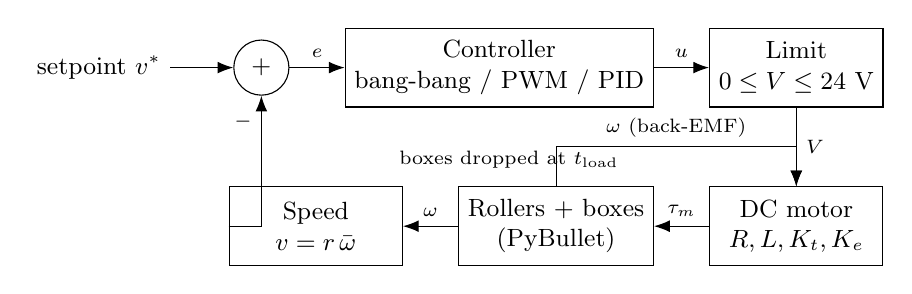
\begin{tikzpicture}[node distance=0.9cm and 0.7cm]
  \node[sum] (sum) {$+$};
  \node[left=0.8cm of sum, font=\small] (sp) {setpoint $v^*$};
  \node[block, right=0.7cm of sum] (ctrl) {Controller\\bang-bang / PWM / PID};
  \node[block, right=0.7cm of ctrl] (sat) {Limit\\$0 \le V \le 24$ V};
  \node[block, below=1.0cm of sat] (motor) {DC motor\\$R, L, K_t, K_e$};
  \node[block, left=0.7cm of motor] (plant) {Rollers + boxes\\(PyBullet)};
  \node[block, left=0.7cm of plant] (sensor) {Speed\\$v = r\,\bar{\omega}$};
  \draw[arr] (sp) -- (sum);
  \draw[arr] (sum) -- node[above,font=\scriptsize]{$e$} (ctrl);
  \draw[arr] (ctrl) -- node[above,font=\scriptsize]{$u$} (sat);
  \draw[arr] (sat) -- node[right,font=\scriptsize]{$V$} (motor);
  \draw[arr] (motor) -- node[above,font=\scriptsize]{$\tau_m$} (plant);
  \draw[arr] (plant) -- node[above,font=\scriptsize]{$\omega$} (sensor);
  \draw[arr] (sensor.west) -| node[pos=0.9,left,font=\scriptsize]{$-$} (sum.south);
  \draw[arr] (plant.north) |- ++(0,0.5) -| node[pos=0.25,above,font=\scriptsize]{$\omega$ (back-EMF)} (motor.north);
  \node[above=0.1cm of plant, xshift=-0.6cm, font=\scriptsize] {boxes dropped at $t_{\text{load}}$};
\end{tikzpicture}
\caption{Block diagram of the conveyor speed control loop}
\label{fig:block}
\end{figure}

\subsection{Conveyor and environment model}

The conveyor is a URDF robot generated at run time: a fixed base link and ten roller links, each a cylinder of radius 5 cm and length 40 cm rotated to lie across the belt, connected to the base by a continuous joint about the $y$ axis and spaced 12 cm apart along $x$. Each roller carries its mass and inertia tensor in the URDF, and the loader is called with the flag that makes PyBullet use the file's inertia; without that flag PyBullet recomputes inertia from the collision shape and gave a value 50 percent too high. PyBullet's built-in joint motors are disabled by commanding zero force in velocity mode, after which raw torques are applied each step.

The load boxes are 20 cm cubes of mass 1 kg with friction coefficient 1.0. A box spans at least two rollers at all times. Boxes are spawned evenly along the belt, 1 cm above the rollers, at $t = 0$ or at a chosen load time. A box whose centre passes the last roller, or whose centre falls below the roller axis, is reset to the start of the belt at rest. A ground plane is loaded 0.5 m below for the rendered view. Figure \ref{fig:pybullet} is a rendered frame.

\begin{figure}[htbp]
\centering
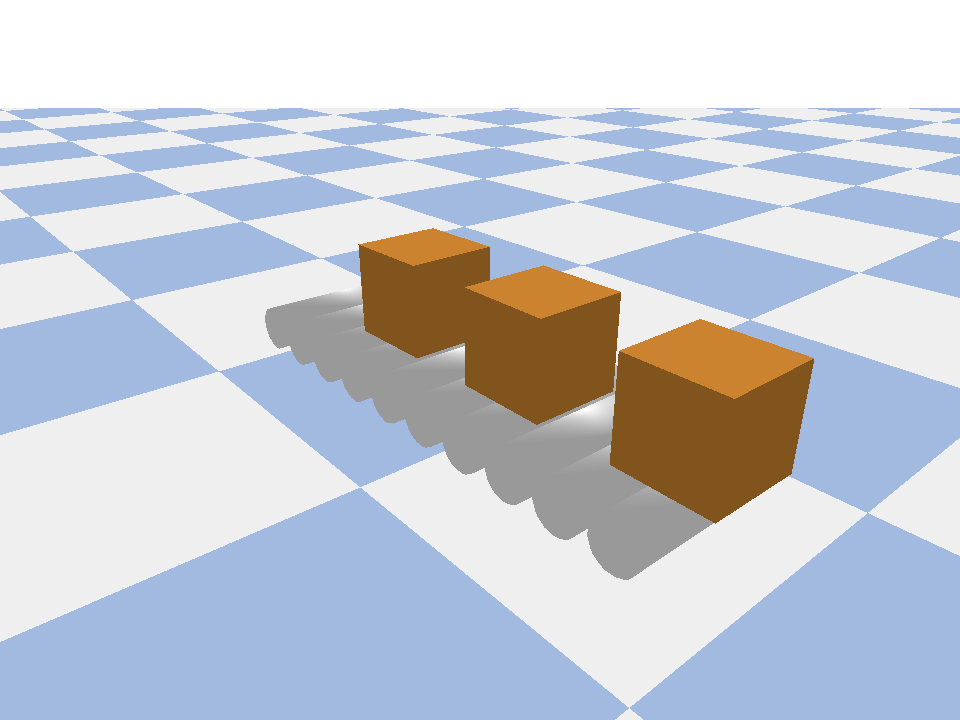
\includegraphics[width=0.75\textwidth]{pybullet.png}
\caption{Rendered view of the ten-roller conveyor with three load boxes}
\label{fig:pybullet}
\end{figure}

\subsection{Sensors and actuators}

The only sensor is the roller joint velocity, read from PyBullet every step and averaged over the ten rollers; multiplied by the radius it is the belt speed. This corresponds to a shaft encoder with a tachometer or differentiated position. The only actuator is the DC motor model of Eq. \ref{eq:motor}, which receives a voltage in $[0, 24]$ V and returns a torque. The torque is divided equally among the ten joints and applied with the roller's own viscous friction subtracted, which keeps the bearing model explicit in the code rather than hidden in URDF damping parameters.

\subsection{Software architecture}

The code is a small Python package, \texttt{conveyor}, with one module per responsibility, shown in Figure \ref{fig:arch} and listed in Table \ref{tab:modules}. The controllers have no dependency on PyBullet and could be run against a real motor driver. The command-line entry point owns the loop and is the only module that imports all the others.

\begin{figure}[htbp]
\centering
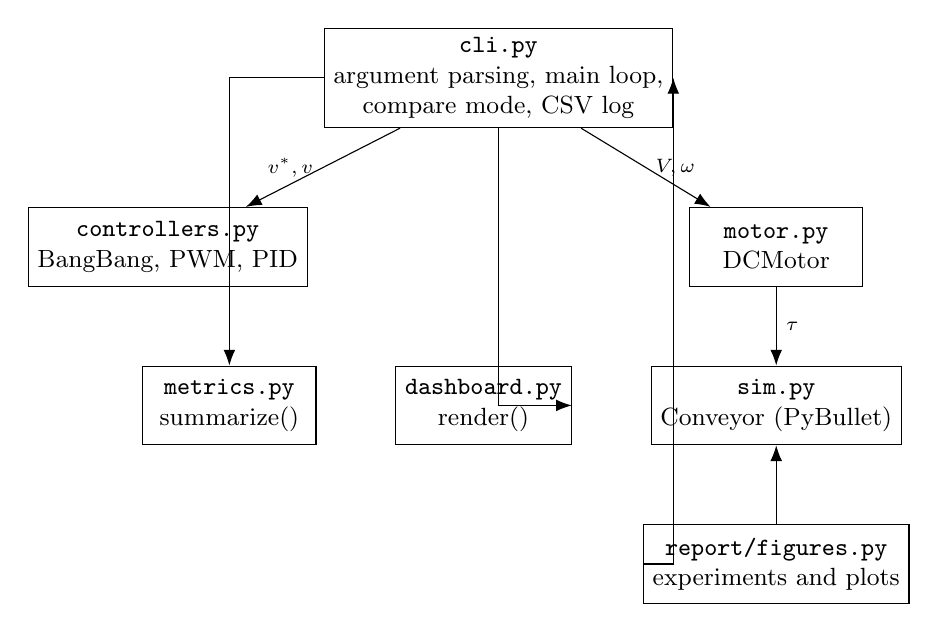
\begin{tikzpicture}[node distance=0.6cm and 1.0cm]
  \node[block, minimum width=3cm] (cli) {\texttt{cli.py}\\argument parsing, main loop,\\compare mode, CSV log};
  \node[block, below left=1.0cm and 0.2cm of cli] (ctrl) {\texttt{controllers.py}\\BangBang, PWM, PID};
  \node[block, below right=1.0cm and 0.2cm of cli] (motor) {\texttt{motor.py}\\DCMotor};
  \node[block, below=1.0cm of motor] (sim) {\texttt{sim.py}\\Conveyor (PyBullet)};
  \node[block, left=1.0cm of sim] (dash) {\texttt{dashboard.py}\\render()};
  \node[block, left=1.0cm of dash] (met) {\texttt{metrics.py}\\summarize()};
  \node[block, below=1.0cm of sim] (fig) {\texttt{report/figures.py}\\experiments and plots};
  \draw[arr] (cli) -- node[left,font=\scriptsize]{$v^*, v$} (ctrl);
  \draw[arr] (cli) -- node[right,font=\scriptsize]{$V, \omega$} (motor);
  \draw[arr] (motor) -- node[right,font=\scriptsize]{$\tau$} (sim);
  \draw[arr] (cli) |- (dash);
  \draw[arr] (cli.west) -| (met);
  \draw[arr] (fig) -| (cli.east);
  \draw[arr] (fig) -- (sim);
\end{tikzpicture}
\caption{Software architecture of the \texttt{conveyor} package}
\label{fig:arch}
\end{figure}

\begin{table}[htbp]
\centering
\caption{Modules of the software and their responsibilities}
\label{tab:modules}
\begin{tabular}{|l|p{9.2cm}|}
\hline
\textbf{Module} & \textbf{Responsibility} \\ \hline
\texttt{sim.py} & Generates the roller URDF, loads it, spawns and recycles boxes, applies torque, exposes speed and $\omega$ \\ \hline
\texttt{motor.py} & DC motor model, voltage in, torque out, holds the 24 V limit \\ \hline
\texttt{controllers.py} & The three control laws behind one \texttt{update(setpoint, speed, dt)} interface \\ \hline
\texttt{dashboard.py} & Text dashboard with bars and a speed sparkline, standard library only \\ \hline
\texttt{metrics.py} & Rise time, overshoot, steady-state error, ripple, load dip, recovery, mean voltage, switches \\ \hline
\texttt{cli.py} & Command-line interface, simulation loop, compare mode, CSV logging \\ \hline
\texttt{report/figures.py} & Runs every experiment of Section 9 and writes the figures \\ \hline
\end{tabular}
\end{table}

\section{Methodology and Algorithms}

\subsection{Overall method}

The work proceeded in five steps. (1) Build the roller conveyor in PyBullet and check that boxes are transported by friction. (2) Add the DC motor model and validate the open-loop plant against Eq. \ref{eq:tf}. (3) Implement the three controllers behind one interface and the dashboard. (4) Tune the PID gains from the model and confirm with a gain sweep. (5) Run the comparison scenarios, generate figures and metrics with one script, and write the report from them. Figure \ref{fig:loop} is the flowchart of the simulation loop that all experiments share.

\begin{figure}[htbp]
\centering
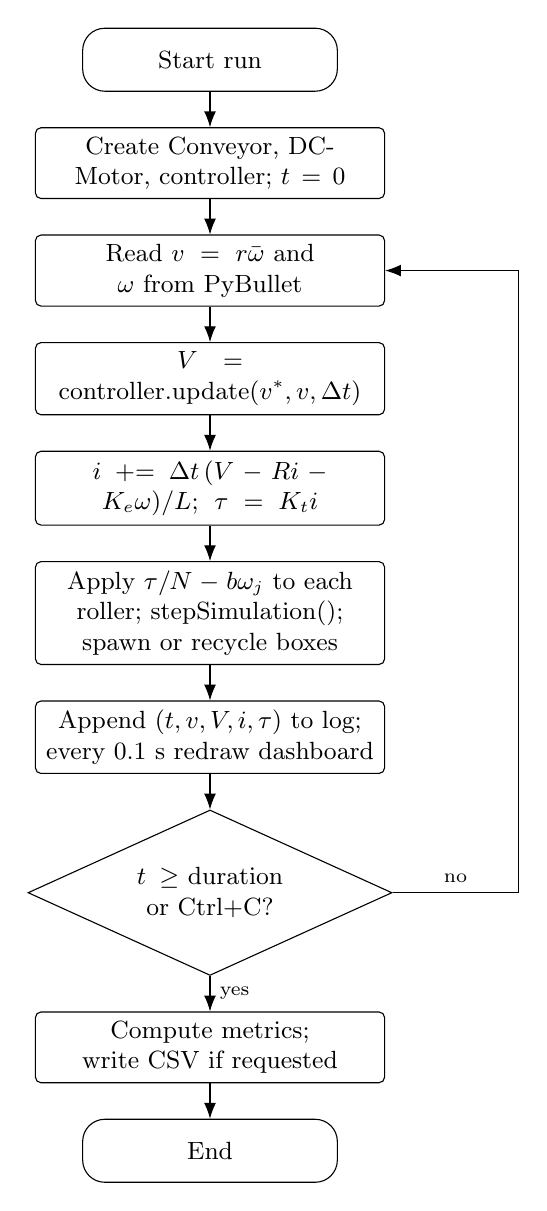
\begin{tikzpicture}[node distance=0.45cm]
  \node[term] (start) {Start run};
  \node[proc, below=of start] (init) {Create Conveyor, DCMotor, controller; $t = 0$};
  \node[proc, below=of init] (read) {Read $v = r\bar{\omega}$ and $\omega$ from PyBullet};
  \node[proc, below=of read] (ctrl) {$V = \text{controller.update}(v^*, v, \Delta t)$};
  \node[proc, below=of ctrl] (motor) {$i \mathrel{+}= \Delta t\,(V - Ri - K_e\omega)/L$;\; $\tau = K_t i$};
  \node[proc, below=of motor] (step) {Apply $\tau/N - b\omega_j$ to each roller; stepSimulation(); spawn or recycle boxes};
  \node[proc, below=of step] (log) {Append $(t, v, V, i, \tau)$ to log; every 0.1 s redraw dashboard};
  \node[dec, below=of log] (done) {$t \ge$ duration or Ctrl+C?};
  \node[proc, below=of done] (sum) {Compute metrics; write CSV if requested};
  \node[term, below=of sum] (end) {End};
  \draw[arr] (start) -- (init);
  \draw[arr] (init) -- (read);
  \draw[arr] (read) -- (ctrl);
  \draw[arr] (ctrl) -- (motor);
  \draw[arr] (motor) -- (step);
  \draw[arr] (step) -- (log);
  \draw[arr] (log) -- (done);
  \draw[arr] (done) -- node[right,font=\scriptsize]{yes} (sum);
  \draw[arr] (done.east) -- ++(1.6,0) node[above,font=\scriptsize,pos=0.5]{no} |- (read.east);
  \draw[arr] (sum) -- (end);
\end{tikzpicture}
\caption{Flowchart of the simulation loop shared by all controllers}
\label{fig:loop}
\end{figure}

\subsection{Bang-bang controller}

The controller keeps one bit of state, whether the motor is on. It turns on when the speed falls below the setpoint minus the hysteresis half-band $h$ and off when it rises above the setpoint plus $h$; inside the band it keeps its state. With $h = 0.02$ m/s this gives a nominal $\pm 4$ percent band around 0.5 m/s. The algorithm is given in Algorithm \ref{alg:bb}.

\begin{algorithm}[htbp]
\caption{Bang-bang speed control with hysteresis}
\label{alg:bb}
\begin{algorithmic}[1]
\State $on \gets$ false, $h \gets 0.02$
\Procedure{update}{$v^*, v, \Delta t$}
  \If{$v < v^* - h$} $on \gets$ true
  \ElsIf{$v > v^* + h$} $on \gets$ false
  \EndIf
  \State \Return $on$ ? $V_{\max}$ : $0$
\EndProcedure
\end{algorithmic}
\end{algorithm}

\subsection{PWM controller}

The PWM controller models a hardware PWM timer. At the start of every carrier period of $T = 20$ ms it samples the error and sets the duty $d = \text{clamp}(K_p e, 0, 1)$ with $K_p = 4$ per m/s, so an error of 0.25 m/s commands full duty. During the period it outputs $V_{\max}$ while the phase is less than $dT$ and 0 afterwards. The duty is held for the whole period, which is the sample-and-hold behaviour of a real timer. See Algorithm \ref{alg:pwm}. Because the duty is proportional to the error, a non-zero duty requires a non-zero error, and the controller settles with an offset: at the operating point the belt needs a mean voltage of about 13 V, that is $d \approx 0.55$, which requires $e \approx 0.14$ m/s at the sampling instant. The error is sampled at the end of the off phase, the trough of the speed ripple, so the time-averaged offset is smaller, about 0.10 m/s in the results.

\begin{algorithm}[htbp]
\caption{Proportional-duty PWM control}
\label{alg:pwm}
\begin{algorithmic}[1]
\State $T \gets 1/50$, $\phi \gets 0$, $d \gets 0$, $K_p \gets 4$
\Procedure{update}{$v^*, v, \Delta t$}
  \If{$\phi = 0$} $d \gets \text{clamp}(K_p (v^* - v), 0, 1)$ \EndIf
  \State $on \gets (\phi < d\,T)$
  \State $\phi \gets \phi + \Delta t$; \textbf{if} $\phi \ge T$ \textbf{then} $\phi \gets 0$
  \State \Return $on$ ? $V_{\max}$ : $0$
\EndProcedure
\end{algorithmic}
\end{algorithm}

\subsection{PID controller with anti-windup}

The PID controller is the textbook discrete form with the integral clamped so that the integral term alone can never exceed $V_{\max}$, Algorithm \ref{alg:pid}. The clamp is the simplest anti-windup scheme in the classification of Peng et al. \cite{peng}. The derivative acts on the raw error difference without filtering, because the measurement is noise-free in simulation; the consequence of that choice when boxes land is discussed in Section 9.5. The output is clamped to $[0, V_{\max}]$, which is the saturation of the actuator.

\begin{algorithm}[htbp]
\caption{PID speed control with integrator clamping}
\label{alg:pid}
\begin{algorithmic}[1]
\State $I \gets 0$, $e_{\text{prev}} \gets$ none, $K_p \gets 40$, $K_i \gets 150$, $K_d \gets 0.5$
\Procedure{update}{$v^*, v, \Delta t$}
  \State $e \gets v^* - v$
  \State $I \gets \text{clamp}(I + e\,\Delta t,\ 0,\ V_{\max}/K_i)$
  \State $D \gets (e_{\text{prev}} = \text{none}) ? 0 : (e - e_{\text{prev}})/\Delta t$; \quad $e_{\text{prev}} \gets e$
  \State \Return $\text{clamp}(K_p e + K_i I + K_d D,\ 0,\ V_{\max})$
\EndProcedure
\end{algorithmic}
\end{algorithm}

\subsection{Controller design and tuning}

The PID gains were chosen from the linear model rather than by trial. The plant has DC gain 0.0385 m/s per volt and a dominant time constant of 77 ms. A proportional gain of $K_p = 40$ V per m/s gives a loop gain of $0.0385 \times 40 = 1.54$, which moves the dominant closed-loop pole to roughly $(1 + 1.54)/0.077 \approx 33$ rad/s, a closed-loop time constant of about 30 ms and a rise of a few tenths of a second once the voltage comes off the limit. The integral gain was then set so that the integrator time constant $K_p/K_i = 0.27$ s is several times slower than the proportional loop, which removes the offset without reintroducing overshoot; $K_i = 150$. A small derivative gain $K_d = 0.5$ was added to damp the response to box impacts. The Routh check of Section 5.5 confirms a large stability margin. Section 9.6 shows the chosen set against a set four times slower and three times faster.

The bang-bang band and the PWM gain were set by the same plant numbers: the band is twice the PID ripple so that both are visible on the same plot, and $K_p = 4$ gives full duty at a quarter of the setpoint, so the PWM controller saturates during the initial ramp like the others and then runs in its linear range.

\subsection{Metrics}

Every run produces a log of $(t, v, V, i, \tau)$ at 1 kHz. From it the following are computed. \textbf{Rise time}: first time the speed reaches 90 percent of the setpoint. \textbf{Overshoot}: peak speed above the setpoint as a percentage of the setpoint. \textbf{Steady-state error}: mean of setpoint minus speed over the last 20 percent of the run. \textbf{Ripple}: peak-to-peak speed over the last 20 percent. \textbf{Load dip}: setpoint minus the minimum speed in the window after the boxes land. \textbf{Recovery}: time after the load change until the speed stays within 0.02 m/s of the setpoint for 0.2 s. \textbf{Mean voltage}: average commanded voltage, a proxy for energy. \textbf{Switches}: number of transitions between zero and non-zero voltage, a proxy for actuator wear.

\section{Simulation Setup}

\textbf{Platform.} PyBullet 3.2.7 in DIRECT (headless) mode for all experiments, with the GUI available for demonstration. Python 3.12 with dependencies managed by \texttt{uv}. Matplotlib only for the report figures. The simulation and controller step is $\Delta t = 1$ ms; the dashboard redraws every 100 steps. Runs are paced to wall-clock time by default and run as fast as possible with \texttt{--fast}. Table \ref{tab:params} lists every parameter.

\begin{table}[htbp]
\centering
\caption{Simulation parameters}
\label{tab:params}
\begin{tabular}{|p{3.6cm}|p{4.0cm}|p{5.6cm}|}
\hline
\textbf{Parameter} & \textbf{Value} & \textbf{Note} \\ \hline
Simulation step $\Delta t$ & 1 ms & controller, motor and physics \\ \hline
Rollers $N$ & 10 & on one shaft, 12 cm pitch \\ \hline
Roller radius $r$, mass $m$ & 0.05 m, 2 kg & $J_1 = 0.0025$ kg\,m$^2$ \\ \hline
Bearing friction $b$ & 0.02 N\,m\,s/rad & per roller, applied in code \\ \hline
Box size, mass, friction & 0.2 m cube, 1 kg, $\mu = 1.0$ & 3 boxes by default \\ \hline
Armature $R$, $L$ & 2 $\Omega$, 0.02 H & $L/R = 10$ ms \\ \hline
$K_t$, $K_e$ & 0.5 N\,m/A, 0.5 V\,s/rad & \\ \hline
Supply limit $V_{\max}$ & 24 V & stall torque 6 N\,m, top speed 0.923 m/s \\ \hline
Bang-bang band $h$ & 0.02 m/s & \\ \hline
PWM $K_p$, carrier & 4 per m/s, 50 Hz & 20 steps per period \\ \hline
PID $K_p, K_i, K_d$ & 40, 150, 0.5 & integral clamp $V_{\max}/K_i$ \\ \hline
Default setpoint & 0.5 m/s & 54 percent of top speed \\ \hline
\end{tabular}
\end{table}

\textbf{How to run.} From a clone of the repository:
\begin{small}
\begin{verbatim}
uv sync                          (macOS: CFLAGS="-Dfdopen=fdopen" uv sync)
uv run conveyor pid --gui        (live dashboard plus 3D window)
uv run conveyor bangbang --setpoint 0.3 --boxes 5
uv run conveyor pwm --duration 5 --fast --log pwm.csv
uv run conveyor pid --load-at 5 --duration 10
uv run conveyor compare --duration 10 --load-at 5
uv sync --group report
uv run python report/figures.py  (regenerates every figure)
\end{verbatim}
\end{small}
The positional argument selects the controller (\texttt{bangbang}, \texttt{pwm}, \texttt{pid} or \texttt{compare}); the flags set the setpoint, duration, number of boxes, the second at which they are dropped, the GUI, pacing and CSV logging. The README in the repository documents each flag and the dashboard rows.

\section{Results and Analysis}

\subsection{Open-loop validation of the plant}

A 24 V step was applied to the motor with no boxes on the belt and the belt speed compared with the response of Eq. \ref{eq:tf} integrated with the same Euler step. Figure \ref{fig:openloop} and Table \ref{tab:openloop} show the agreement. The final speed matches to four digits and the 63 percent time to within 3 percent, which meets Objective 2 and confirms that the roller inertia, friction and motor coupling in PyBullet are what the equations say they are. This check is what revealed the URDF inertia issue described in Section 6.2: before the loader flag was set, the simulated time constant was 0.121 s instead of 0.079 s.

\begin{figure}[htbp]
\centering
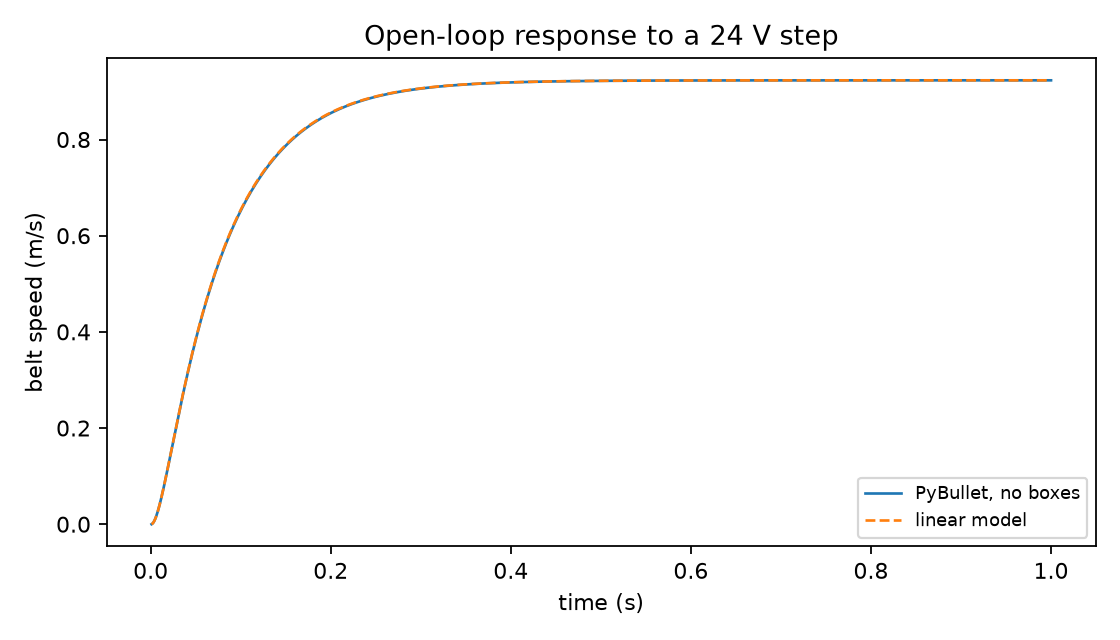
\includegraphics[width=0.85\textwidth]{openloop.png}
\caption{Open-loop belt speed for a 24 V step: PyBullet plant against the linear model}
\label{fig:openloop}
\end{figure}

\begin{table}[htbp]
\centering
\caption{Open-loop validation against the linear model}
\label{tab:openloop}
\begin{tabular}{|l|c|c|}
\hline
\textbf{Quantity} & \textbf{Linear model} & \textbf{PyBullet} \\ \hline
Final belt speed at 24 V (m/s) & 0.9231 & 0.9231 \\ \hline
Time to 63 percent of final (s) & 0.077 & 0.079 \\ \hline
DC gain (m/s per V) & 0.0385 & 0.0385 \\ \hline
\end{tabular}
\end{table}

\begin{figure}[htbp]
\centering
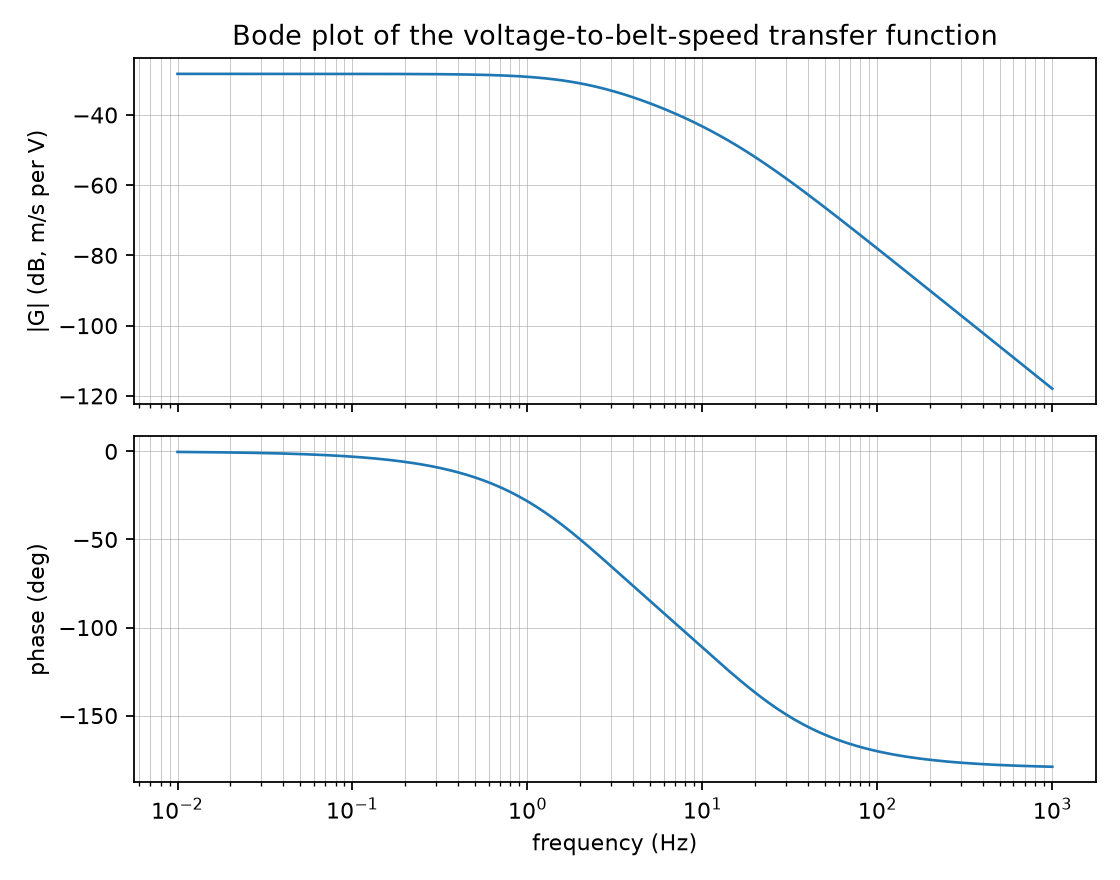
\includegraphics[width=0.85\textwidth]{bode.png}
\caption{Bode plot of the voltage-to-belt-speed transfer function of Eq. \ref{eq:tf}}
\label{fig:bode}
\end{figure}

\subsection{Step response with load present}

Figure \ref{fig:step} shows the three controllers stepping to 0.5 m/s with three boxes resting on the belt from the start, and Table \ref{tab:step} the metrics over a 6 s run. The two switching controllers apply full voltage from the first step and reach 90 percent of the setpoint in about 70 ms, limited only by the plant. PID starts at $K_p e = 20$ V, backs off as the error shrinks, and reaches 90 percent in 0.49 s with 1.9 percent overshoot; it then holds the setpoint with a mean error of a few $10^{-6}$ m/s. Bang-bang holds a mean error of 0.003 m/s but with a ripple of 0.074 m/s peak-to-peak, which is wider than the $\pm 0.02$ band because the plant keeps accelerating for a few milliseconds after each switch. PWM never reaches 90 percent of the setpoint: it settles at 0.40 m/s, the proportional offset predicted in Section 7.3, with a ripple of 0.035 m/s. The mean voltage is about 13.4 V for the two controllers that reach the setpoint and 10.9 V for PWM, which is simply the voltage needed for the lower speed it settles at. In 6 s bang-bang switched 270 times and PWM 595 times.

\begin{figure}[htbp]
\centering
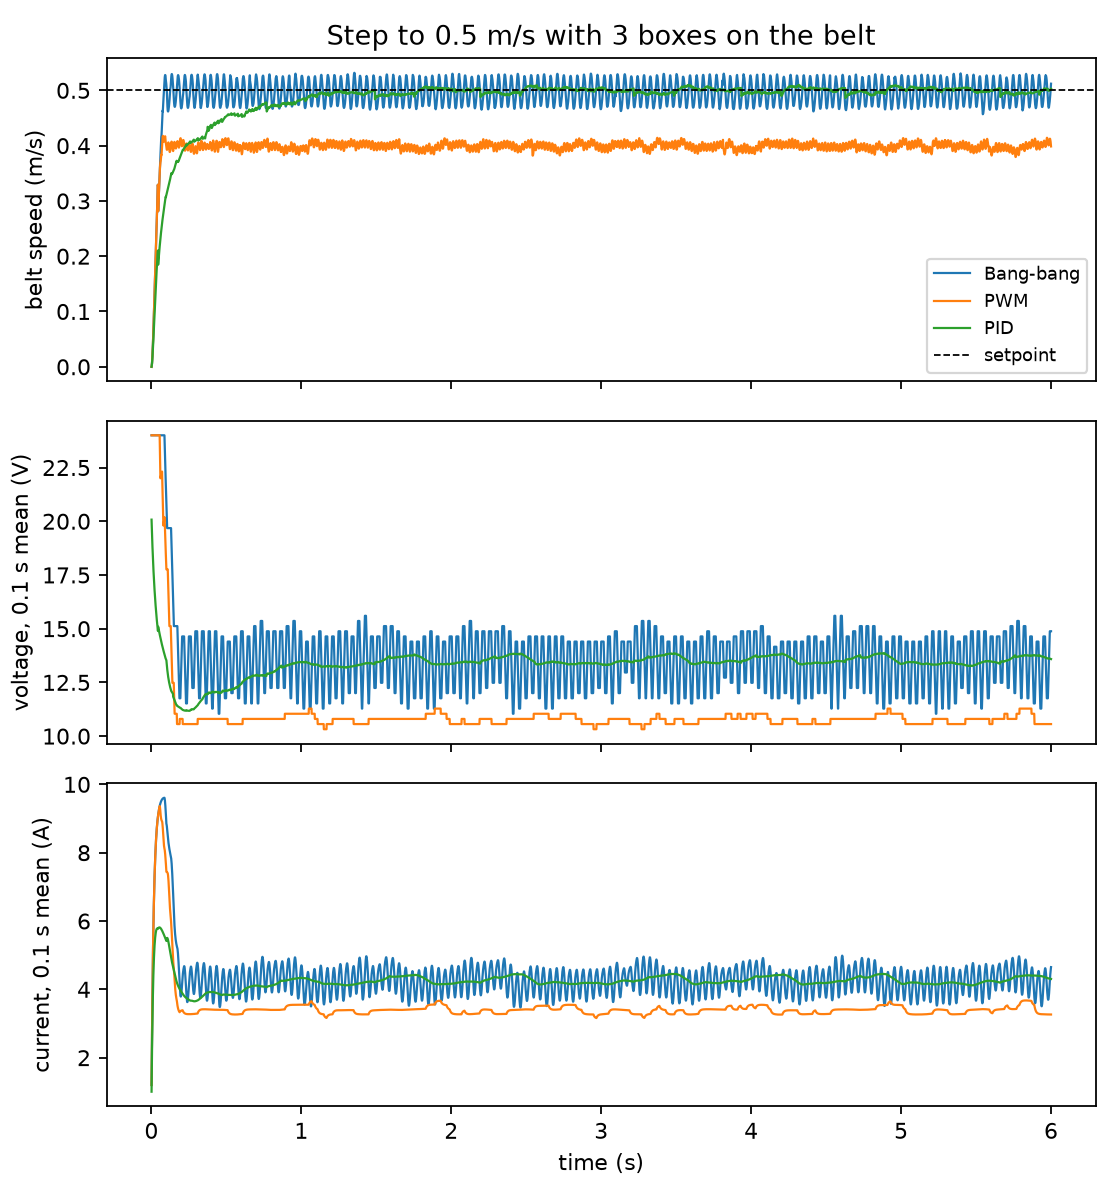
\includegraphics[width=0.9\textwidth]{step.png}
\caption{Step to 0.5 m/s with three boxes on the belt: belt speed, 0.1 s mean voltage and 0.1 s mean current}
\label{fig:step}
\end{figure}

\begin{table}[htbp]
\centering
\caption{Step response metrics, setpoint 0.5 m/s, three boxes from $t = 0$, 6 s run}
\label{tab:step}
\begin{tabular}{|l|c|c|c|}
\hline
\textbf{Metric} & \textbf{Bang-bang} & \textbf{PWM} & \textbf{PID} \\ \hline
Rise time to 90 percent (s) & 0.073 & not reached & 0.488 \\ \hline
Overshoot (percent) & 6.3 & 0.0 & 1.9 \\ \hline
Steady-state error (m/s) & 0.0035 & 0.1012 & 0.0000 \\ \hline
Ripple, peak-to-peak (m/s) & 0.074 & 0.035 & 0.021 \\ \hline
Mean voltage (V) & 13.60 & 10.88 & 13.35 \\ \hline
Switches in 6 s & 270 & 595 & 0 \\ \hline
\end{tabular}
\end{table}

\subsection{Switching detail}

Figure \ref{fig:switching} zooms into 0.2 s of the bang-bang and PWM runs. The PWM voltage is a regular 50 Hz pulse train with the duty changing only at period boundaries; the bang-bang voltage switches whenever the speed crosses the band, at about 46 Hz here, with pulses of unequal length. The current traces show the electrical filtering: with $L/R = 10$ ms the current cannot follow the 24 V edges and ramps up and down by several amps, going negative in the bang-bang off phases because the shorted armature brakes. The speed traces show the mechanical filtering on top: the bang-bang speed swings by about 0.07 m/s around the setpoint, while the PWM speed carries only a 0.03 m/s ripple but sits 0.1 m/s low. This figure is the direct evidence for the actuation theory of Section 5.4.

\begin{figure}[htbp]
\centering
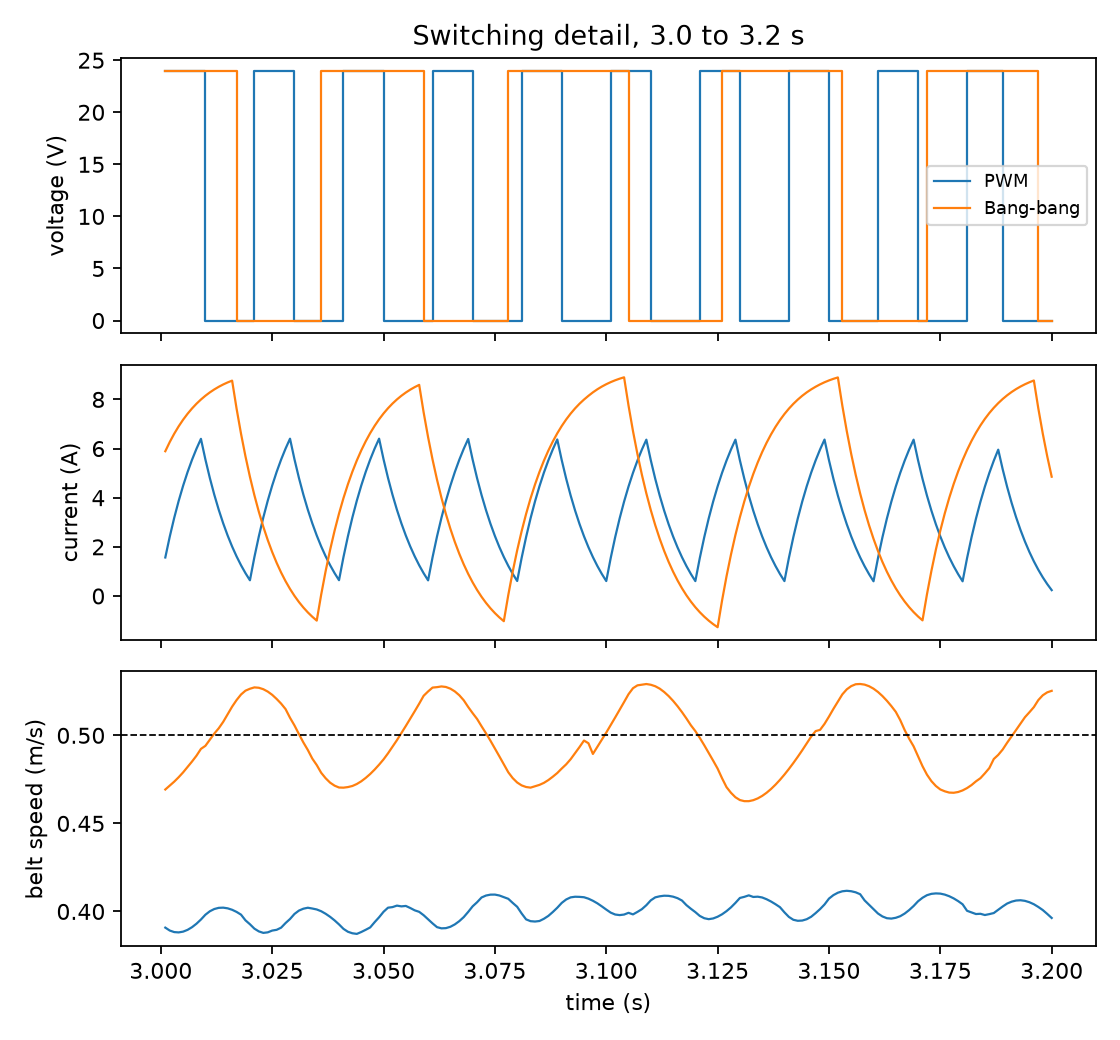
\includegraphics[width=0.9\textwidth]{switching.png}
\caption{Voltage, current and belt speed for bang-bang and PWM over 0.2 s at steady state}
\label{fig:switching}
\end{figure}

\subsection{Load change}

In the load scenario the belt runs empty for 5 s and three boxes are then dropped onto it at once, after which the normal recycling continues. Figure \ref{fig:load} and Table \ref{tab:load} give the results over 10 s. Bang-bang dips by 0.088 m/s and then returns to its limit cycle; because the limit cycle is wider than the 0.02 m/s recovery band, no recovery time is defined for it, which is an honest statement of what it does: it never settles. PWM dips by 0.158 m/s, the largest of the three, because its duty can only rise when the error rises, and it then settles at a slightly lower offset than before since the load torque has increased. PID dips by 0.064 m/s, the smallest, and is back inside the band in 0.123 s. The voltage traces after the load change show the mean voltage for all three rising from about 10 V to 13 V, which is the extra voltage needed to supply the friction torque of the boxes at speed. The small periodic bumps in the PID trace after 5 s are boxes leaving the end and being re-dropped at the start.

\begin{figure}[htbp]
\centering
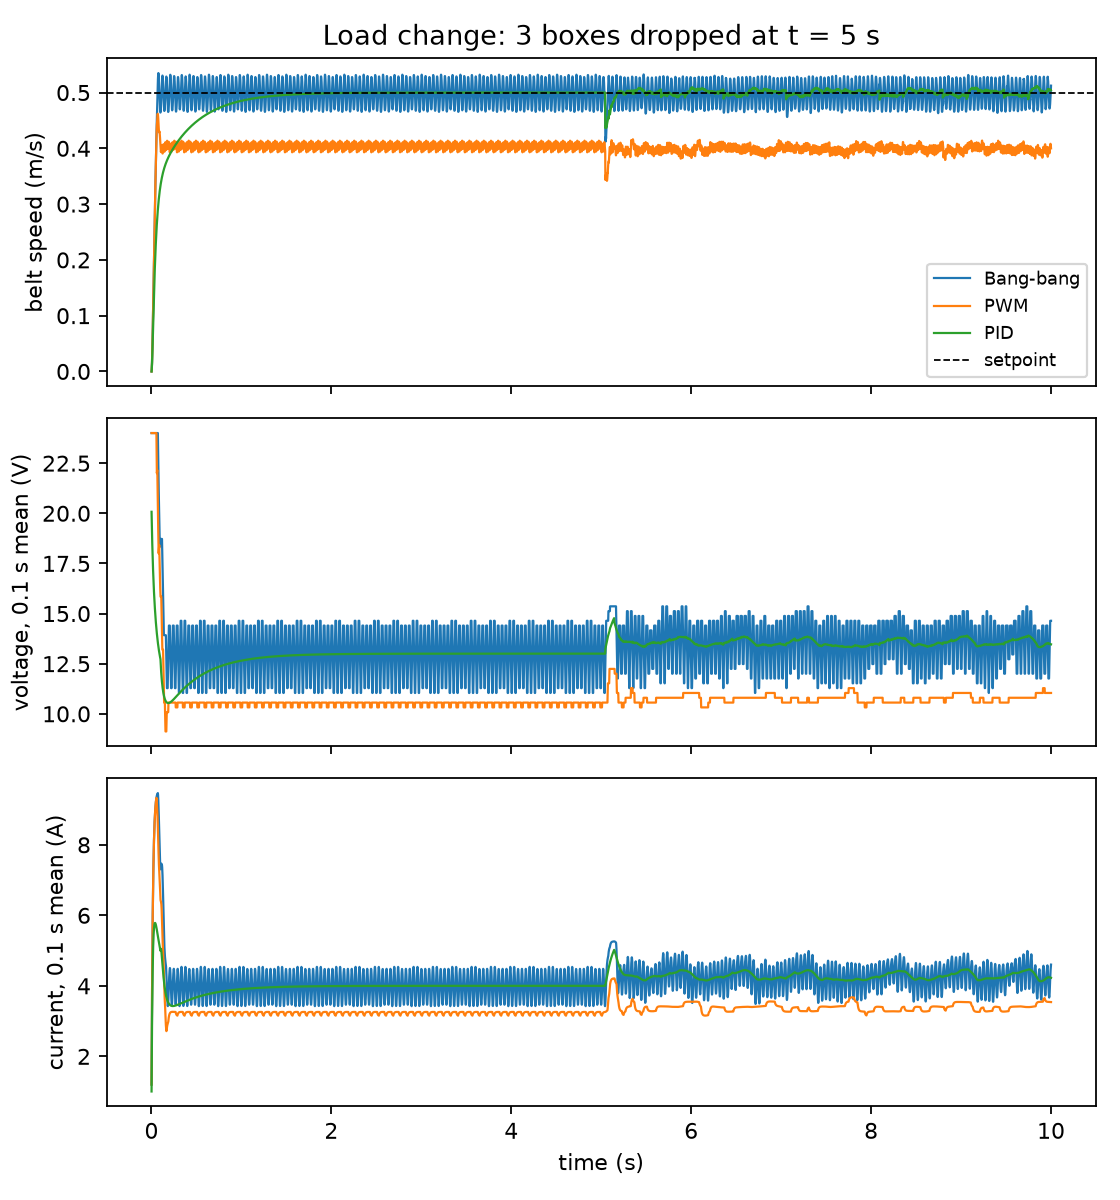
\includegraphics[width=0.9\textwidth]{load.png}
\caption{Load change: three boxes dropped at $t = 5$ s onto a belt running at 0.5 m/s}
\label{fig:load}
\end{figure}

\begin{table}[htbp]
\centering
\caption{Load-change metrics, three boxes dropped at $t = 5$ s, 10 s run}
\label{tab:load}
\begin{tabular}{|l|c|c|c|}
\hline
\textbf{Metric} & \textbf{Bang-bang} & \textbf{PWM} & \textbf{PID} \\ \hline
Load dip (m/s) & 0.088 & 0.158 & 0.064 \\ \hline
Recovery to $\pm 0.02$ m/s (s) & never & never & 0.123 \\ \hline
Steady-state error after load (m/s) & 0.0031 & 0.1013 & 0.0004 \\ \hline
Ripple after load (m/s) & 0.069 & 0.035 & 0.024 \\ \hline
Mean voltage over run (V) & 13.30 & 10.70 & 13.17 \\ \hline
Switches in 10 s & 456 & 995 & 0 \\ \hline
\end{tabular}
\end{table}

\subsection{Actuator saturation and anti-windup}

Figure \ref{fig:saturation} shows the PID controller at setpoints of 0.5, 0.8 and 1.1 m/s, the last of which is above the 0.923 m/s top speed. At 0.5 and 0.8 m/s the voltage comes off the 24 V limit within 0.1 s and the belt settles on the setpoint with mean voltages of 13.3 V and 21.4 V (Table \ref{tab:sat}). At 1.1 m/s the voltage stays pinned at 24 V, the belt runs at about 0.9 m/s and the error never closes; the controller is doing all it can and the steady-state error of 0.18 m/s is a property of the actuator, not of the controller. This run also shows a side effect that was not planned: at 0.9 m/s the boxes are thrown off the end roughly once a second and re-dropped, and each landing produces a speed jump that the unfiltered derivative term turns into a voltage spike of several volts, visible as the narrow dips in the voltage trace. A derivative filter or a derivative on the measurement would remove this and is listed as future work.

\begin{figure}[htbp]
\centering
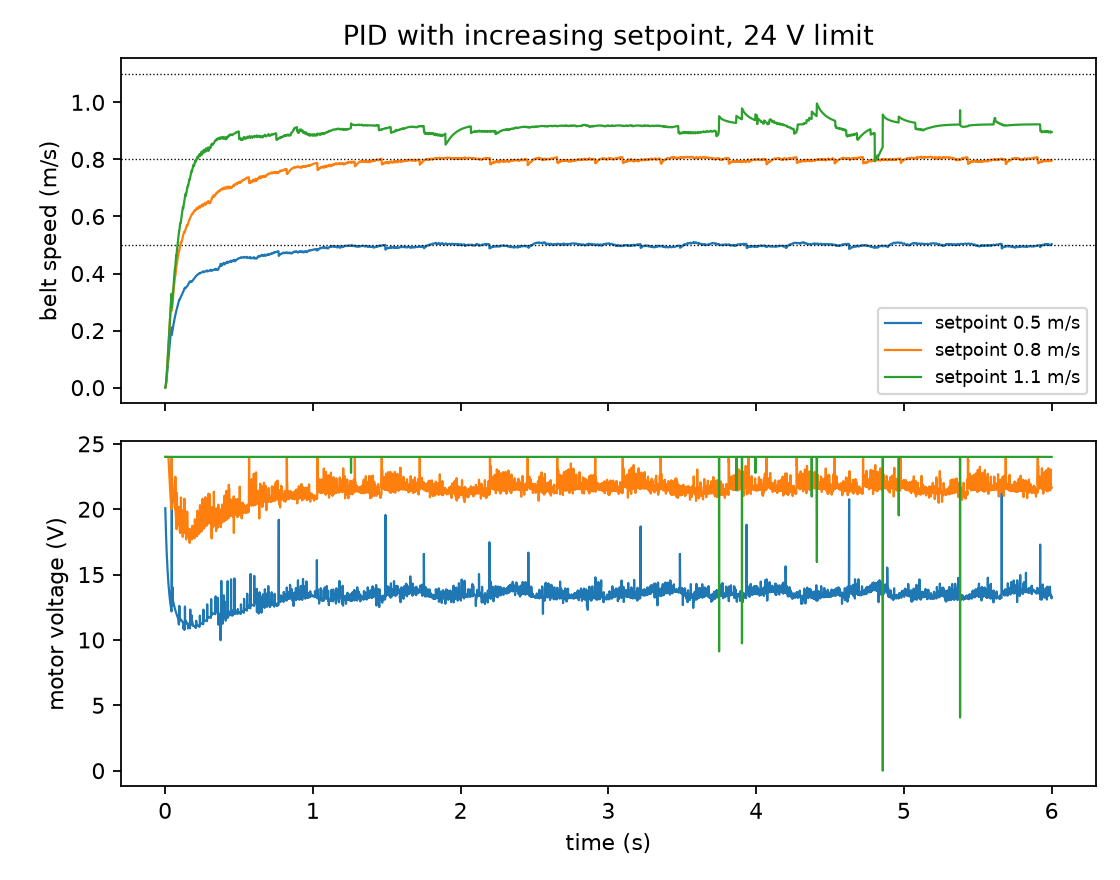
\includegraphics[width=0.9\textwidth]{saturation.png}
\caption{PID at three setpoints; at 1.1 m/s the 24 V limit is reached and the setpoint cannot be met}
\label{fig:saturation}
\end{figure}

\begin{table}[htbp]
\centering
\caption{PID under increasing setpoint with a 24 V limit}
\label{tab:sat}
\begin{tabular}{|l|c|c|c|}
\hline
\textbf{Setpoint (m/s)} & \textbf{0.5} & \textbf{0.8} & \textbf{1.1} \\ \hline
Rise time to 90 percent (s) & 0.488 & 0.498 & not reached \\ \hline
Overshoot (percent) & 1.9 & 1.2 & 0.0 \\ \hline
Steady-state error (m/s) & 0.0000 & $-0.0003$ & 0.183 \\ \hline
Mean voltage (V) & 13.35 & 21.37 & 23.98 \\ \hline
\end{tabular}
\end{table}

Wind-up is demonstrated in Figure \ref{fig:windup}. The setpoint is held at an unreachable 1.2 m/s for 3 s, so the voltage saturates at 24 V and the integral term accumulates, and is then dropped to 0.5 m/s. With the integrator clamped at $V_{\max}/K_i$, the voltage falls to zero on the instant of the setpoint change, the motor brakes, and the belt is at 0.5 m/s within 0.77 s. Without the clamp the integral has grown far beyond what the output can use, the voltage stays at 24 V for a further two seconds while the integral unwinds, and the belt reaches 0.5 m/s only after 3.03 s (Table \ref{tab:windup}). This is the classic wind-up behaviour described by Åström and Murray \cite{astrom-murray} and the reason every industrial PID carries an anti-windup scheme.

\begin{figure}[htbp]
\centering
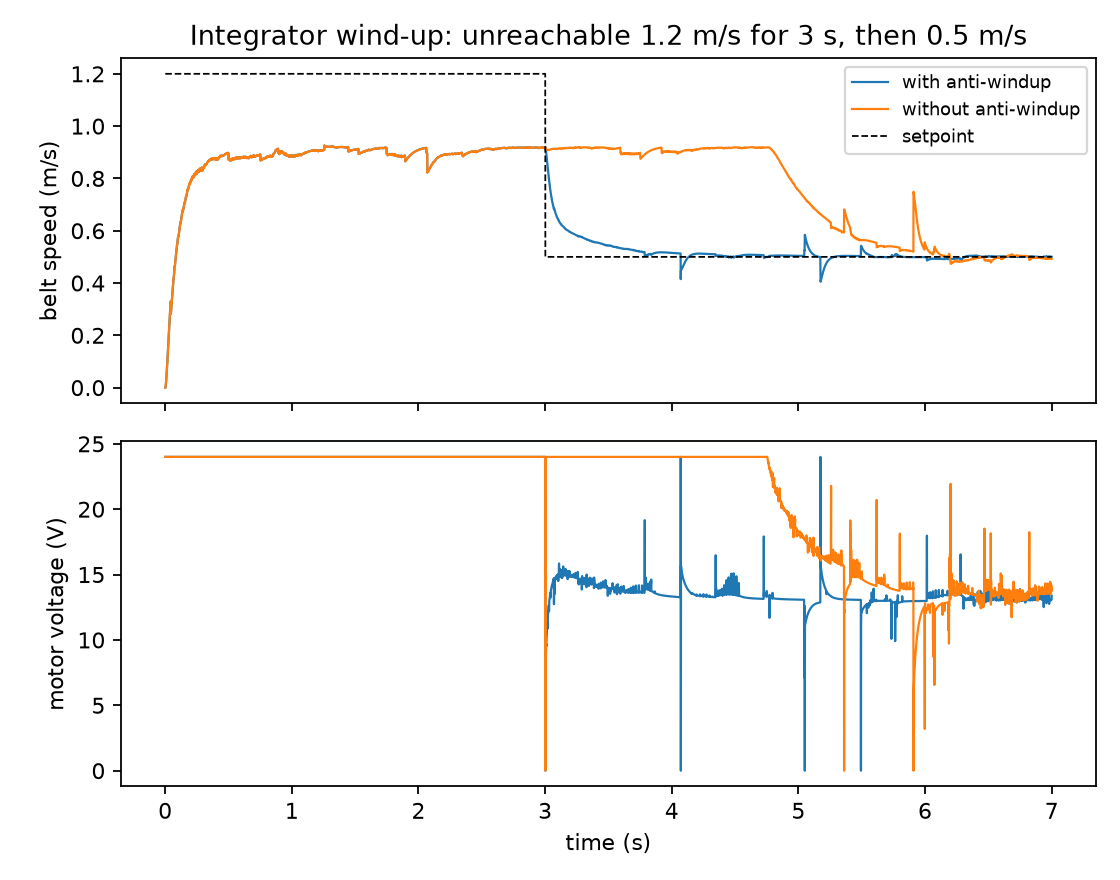
\includegraphics[width=0.9\textwidth]{windup.png}
\caption{Integrator wind-up: unreachable setpoint for 3 s, then a drop to 0.5 m/s, with and without the integral clamp}
\label{fig:windup}
\end{figure}

\begin{table}[htbp]
\centering
\caption{Effect of anti-windup after 3 s of saturation}
\label{tab:windup}
\begin{tabular}{|l|c|c|}
\hline
\textbf{Quantity} & \textbf{With clamp} & \textbf{Without clamp} \\ \hline
Time to reach 0.5 m/s after the drop (s) & 0.77 & 3.03 \\ \hline
Voltage immediately after the drop (V) & 0 & 24 \\ \hline
\end{tabular}
\end{table}

\subsection{PID gain sensitivity}

Figure \ref{fig:tuning} and Table \ref{tab:tuning} compare the chosen gains with a slow set and an aggressive set on the same step. The slow set ($K_p = 10$, $K_i = 20$, no derivative) never saturates, takes 3.4 s to reach 90 percent and still carries a 0.05 m/s error at 4 s because its integrator is slow. The aggressive set ($K_p = 120$, $K_i = 600$) rises in 78 ms, as fast as bang-bang, with 1.3 percent overshoot, but its voltage trace is noticeably noisier because the high proportional gain amplifies every speed fluctuation caused by the boxes. The chosen set is a compromise: a rise of 0.49 s is acceptable for a conveyor, the overshoot is below 2 percent and the control effort is smooth. All three sets are far inside the Routh stability bound of Section 5.5, which is consistent with the absence of any oscillatory tendency in the plots.

\begin{figure}[htbp]
\centering
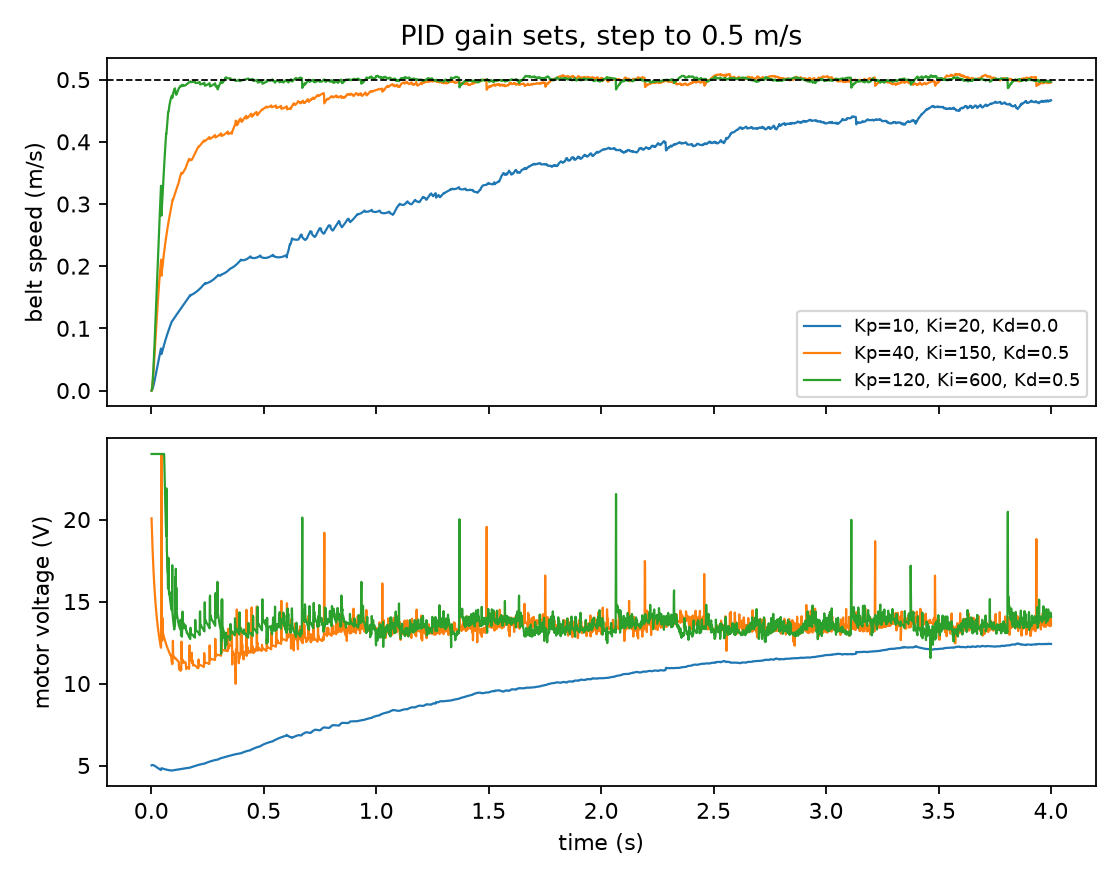
\includegraphics[width=0.9\textwidth]{tuning.png}
\caption{Three PID gain sets on the step to 0.5 m/s}
\label{fig:tuning}
\end{figure}

\begin{table}[htbp]
\centering
\caption{PID gain sensitivity on the 0.5 m/s step, 4 s run}
\label{tab:tuning}
\begin{tabular}{|l|c|c|c|}
\hline
\textbf{Gains $(K_p, K_i, K_d)$} & \textbf{(10, 20, 0)} & \textbf{(40, 150, 0.5)} & \textbf{(120, 600, 0.5)} \\ \hline
Rise time (s) & 3.44 & 0.49 & 0.08 \\ \hline
Overshoot (percent) & 0.0 & 1.8 & 1.3 \\ \hline
Error at end of run (m/s) & 0.049 & 0.001 & 0.000 \\ \hline
Mean voltage (V) & 9.72 & 13.25 & 13.73 \\ \hline
\end{tabular}
\end{table}

\subsection{Discussion}

\textbf{What worked.} The physics plant matches the analytical model, so the comparison rests on a plant whose behaviour is understood rather than merely observed. The three controllers behave as theory predicts: bang-bang is fastest but never settles and switches continuously; PWM with a proportional duty is smooth but carries a load-dependent offset; PID is slower on the first step but has no offset, the smallest dip and the fastest recovery under a load change. The anti-windup experiment produced a four-fold difference in recovery time from a single line of code, which is a strong argument for the practice. The dashboard made tuning fast: the sparkline shows ripple and settling at a glance, and the compare table turns a visual impression into numbers.

\textbf{What did not, or only partly.} The PWM carrier is 50 Hz rather than the kilohertz of a real drive, because the physics step is 1 ms and a faster carrier would have too few steps per period for a usable duty resolution. This makes the PWM current ripple much larger than in practice and is the main fidelity limit of the study. The unfiltered derivative term reacts to box impacts with voltage spikes, harmless here but a sign that a real implementation needs a derivative filter. The PID rise time is set by how fast the voltage comes off the limit, and a feed-forward term computed from the model would shorten it without touching the gains. Finally, the recovery-time metric is undefined for the switching controllers because their ripple exceeds the band; a wider band would give a number but would hide the fact that they never truly settle.

\section{Contribution}

Table \ref{tab:contrib} lists the technical contribution of each member. Each claim is traceable to commits in the group repository or to a part of the demonstration video. Each member signs his or her own row in the printed copy. Who wrote which section of this report is given in the Writing Allocation table after the Index.

\begin{table}[htbp]
\centering
\caption{Technical contribution of each member}
\label{tab:contrib}
\begin{tabular}{|c|p{2.9cm}|p{6.1cm}|p{2.0cm}|}
\hline
\textbf{S. No.} & \textbf{Name and SAP ID} & \textbf{Technical contribution} & \textbf{Signature} \\ \hline
1 & Amulya Jain (500122439) & Built the PyBullet conveyor: generated roller URDF, joint torque application, box spawning, recycling and load-at timing in \texttt{sim.py}; found and fixed the URDF inertia loading issue; rendered Figure \ref{fig:pybullet}. & \\[0.6cm] \hline
2 & Aasthik Upadhyay (500123174) & DC motor model in \texttt{motor.py}; derived the transfer function and Bode plot; open-loop validation experiment and Figures \ref{fig:openloop}, \ref{fig:bode}. & \\[0.6cm] \hline
3 & Krish Manwani (500123449) & Bang-bang and PWM controllers in \texttt{controllers.py}; switching-detail experiment and Figure \ref{fig:switching}; literature and industry review. & \\[0.6cm] \hline
4 & Vanshaj Tiwari (500123258) & PID controller with integrator clamp; model-based tuning and gain sweep; saturation and wind-up experiments, Figures \ref{fig:saturation} to \ref{fig:tuning}. & \\[0.6cm] \hline
5 & Yash Dagar (500125147) & Command-line interface, dashboard and metrics (\texttt{cli.py}, \texttt{dashboard.py}, \texttt{metrics.py}); \texttt{report/figures.py} pipeline; repository, README and build setup. & \\[0.6cm] \hline
\end{tabular}
\end{table}

\section{Co-learning Reflection}

% Each member should rewrite his or her paragraph in his or her own words before printing.

\textbf{Amulya Jain.} I learned on my own how PyBullet describes a robot in URDF, how joints, inertia and friction are set, and that the engine does not trust the inertia in the file unless told to; finding that bug taught me to always check a simulation against a hand calculation. From Aasthik I learned how the motor equations connect to what the rollers do. I taught the others how to inspect dynamics information and contact points in PyBullet while debugging the box recycling.

\textbf{Aasthik Upadhyay.} I taught myself the DC motor model from the drives textbooks and how to turn two coupled first-order equations into one transfer function and a Bode plot. Vanshaj showed me how the closed-loop characteristic polynomial comes out of that transfer function and how the Routh condition is applied. I explained back-EMF and why current goes negative when the voltage is switched off to the whole team, which changed how we read the current plots.

\textbf{Krish Manwani.} I learned on my own how hysteresis controllers produce a limit cycle and how a PWM timer samples and holds a duty cycle. Yash taught me how the common controller interface lets a new control law drop into the loop without touching anything else. I taught the team the difference between PWM as an actuation method and the control law that sets the duty, which is what explains the offset in our results.

\textbf{Vanshaj Tiwari.} I learned PID tuning from the plant model rather than by trial, and I learned what integrator wind-up looks like in practice when I ran the setpoint-drop experiment. Amulya helped me understand why the boxes cause the voltage spikes in the saturation run. I taught the others how to read the metrics table and why recovery time is undefined for the switching controllers.

\textbf{Yash Dagar.} I learned how to keep a simulation, a dashboard and a figure pipeline reproducible from one repository with \texttt{uv}, and how to make a terminal dashboard refresh in place with nothing but the standard library. Krish taught me the switching behaviour I was plotting. I taught the team how to set up the project, run the compare mode and regenerate every figure in this report from the script.

\section{Conclusion and Future Scope}

A brushed DC motor driving a ten-roller conveyor with rigid load boxes was built in PyBullet, validated against its analytical transfer function, and controlled with bang-bang, PWM and PID speed controllers from one command-line tool with a live dashboard. On a step to 0.5 m/s with three boxes, bang-bang reached the setpoint in 73 ms but oscillated with a 0.074 m/s ripple and switched 45 times a second; proportional-duty PWM settled 0.10 m/s low; PID reached the setpoint in 0.49 s with 1.9 percent overshoot and no offset. When three boxes were dropped onto a running belt, PID dipped least (0.064 m/s) and recovered in 0.12 s, while the other two dipped more and never settled inside the band. The 24 V limit was shown to cap the belt at 0.92 m/s regardless of the controller, and integrator clamping cut the recovery after a saturated period from 3.0 s to 0.8 s. All five objectives of Section 2 were met.

For industry the results say what drive engineers know but rarely measure on one plant: on-off control is acceptable only where speed ripple does not matter, open-loop or proportional PWM cannot hold a speed under a varying load, and a PID loop with anti-windup is the minimum for a conveyor that feeds timed downstream equipment. Moving the work to a real roller conveyor would need three additions: a current loop inside the speed loop so that the switching stage can be driven at kilohertz with current limiting, a derivative filter or derivative-on-measurement to stop impacts from kicking the output, and an encoder model with quantisation and noise so that the gains are tuned on a realistic measurement. Feed-forward from the model would shorten the PID rise time, and a belt with compliance and slip between rollers would be the next step in plant fidelity.

\begin{thebibliography}{99}
\addcontentsline{toc}{section}{References}
\bibitem{cema} Conveyor Equipment Manufacturers Association, \textit{Belt Conveyors for Bulk Materials}, 7th ed. Naples, FL, USA: CEMA, 2014.
\bibitem{hughes} A. Hughes and B. Drury, \textit{Electric Motors and Drives: Fundamentals, Types and Applications}, 5th ed. Oxford, UK: Newnes, 2019.
\bibitem{mohan} N. Mohan, T. M. Undeland, and W. P. Robbins, \textit{Power Electronics: Converters, Applications, and Design}, 3rd ed. Hoboken, NJ, USA: Wiley, 2003.
\bibitem{leonhard} W. Leonhard, \textit{Control of Electrical Drives}, 3rd ed. Berlin, Germany: Springer, 2001.
\bibitem{astrom-hagglund} K. J. Åström and T. Hägglund, \textit{Advanced PID Control}. Research Triangle Park, NC, USA: ISA, 2006.
\bibitem{pybullet} E. Coumans and Y. Bai, ``PyBullet, a Python module for physics simulation for games, robotics and machine learning,'' 2016--2021. [Online]. Available: http://pybullet.org
\bibitem{ogata} K. Ogata, \textit{Modern Control Engineering}, 5th ed. Upper Saddle River, NJ, USA: Prentice Hall, 2010.
\bibitem{franklin} G. F. Franklin, J. D. Powell, and A. Emami-Naeini, \textit{Feedback Control of Dynamic Systems}, 8th ed. Harlow, UK: Pearson, 2019.
\bibitem{astrom-murray} K. J. Åström and R. M. Murray, \textit{Feedback Systems: An Introduction for Scientists and Engineers}, 2nd ed. Princeton, NJ, USA: Princeton University Press, 2021.
\bibitem{krishnan} R. Krishnan, \textit{Electric Motor Drives: Modeling, Analysis, and Control}. Upper Saddle River, NJ, USA: Prentice Hall, 2001.
\bibitem{ziegler} J. G. Ziegler and N. B. Nichols, ``Optimum settings for automatic controllers,'' \textit{Transactions of the ASME}, vol. 64, pp. 759--768, 1942.
\bibitem{peng} Y. Peng, D. Vrančić, and R. Hanus, ``Anti-windup, bumpless, and conditioned transfer techniques for PID controllers,'' \textit{IEEE Control Systems Magazine}, vol. 16, no. 4, pp. 48--57, 1996.
\end{thebibliography}

\clearpage
\section*{Appendix: Links and Logs}
\addcontentsline{toc}{section}{Appendix: Links and Logs}

\textbf{GitHub repository:} \url{https://github.com/yashdagar/conveyor-motor-speed-control}

\textbf{YouTube video (Unlisted):} \underline{\hspace{8cm}}

\subsection*{Meeting log}
\begin{center}
\begin{tabular}{|c|p{2.2cm}|p{1.8cm}|p{2.4cm}|p{5.4cm}|}
\hline
\textbf{No.} & \textbf{Date} & \textbf{Duration} & \textbf{Attendees} & \textbf{Decisions} \\ \hline
1 & & & & \\[0.5cm] \hline
2 & & & & \\[0.5cm] \hline
3 & & & & \\[0.5cm] \hline
4 & & & & \\[0.5cm] \hline
5 & & & & \\[0.5cm] \hline
\end{tabular}
\end{center}

\subsection*{Peer-assessment sheets}
One sheet per member, filled individually for every team-mate (format from the Project Instructions, Section 4).

\newcommand{\peersheet}[1]{%
\begin{minipage}{\textwidth}
\textbf{Filled by: #1}\\[0.2cm]
\begin{tabular}{|c|p{3.8cm}|p{1.9cm}|p{1.9cm}|p{2.0cm}|p{1.9cm}|}
\hline
\textbf{No.} & \textbf{Team-mate name and SAP ID} & \textbf{Contri\-bution (1-5)} & \textbf{Reliability (1-5)} & \textbf{Helped others learn (1-5)} & \textbf{Quality of work (1-5)} \\ \hline
1 & & & & & \\[0.3cm] \hline
2 & & & & & \\[0.3cm] \hline
3 & & & & & \\[0.3cm] \hline
4 & & & & & \\[0.3cm] \hline
\end{tabular}
\end{minipage}\\[0.6cm]}

\peersheet{Amulya Jain (500122439)}
\peersheet{Aasthik Upadhyay (500123174)}
\peersheet{Krish Manwani (500123449)}
\peersheet{Vanshaj Tiwari (500123258)}
\peersheet{Yash Dagar (500125147)}

\end{document}
